\documentclass[a4paper,11pt]{article}

% === JCAP-like formatting ===
\usepackage[utf8]{inputenc}
\usepackage[T1]{fontenc}
\usepackage{amsmath,amssymb,amsfonts}
\usepackage{mathtools}
\usepackage{graphicx}
\usepackage{hyperref}
\usepackage{xcolor}
\usepackage{booktabs}
\usepackage{multirow}
\usepackage{enumitem}
\usepackage[margin=2.5cm]{geometry}

\hypersetup{colorlinks=true,linkcolor=blue!60!black,citecolor=green!50!black,urlcolor=blue!70!black}

% === Custom commands ===
\newcommand{\MPl}{M_{\rm Pl}}
\newcommand{\LCDM}{$\Lambda$CDM}
\newcommand{\chif}{\chi}
\newcommand{\phif}{\varphi}
\newcommand{\fchi}{f_\chi}
\newcommand{\fphi}{f_\varphi}
\newcommand{\Lchi}{\Lambda_\chi}
\newcommand{\lag}{\lambda_g}
\newcommand{\gBL}{g_{B\text{-}L}}
\newcommand{\UBL}{\mathrm{U}(1)_{B\text{-}L}}
\newcommand{\SUt}{\mathrm{SU}(2)}
\newcommand{\etaB}{\eta_B}
\newcommand{\e}[1]{\times 10^{#1}}

% ======================================================================
\begin{document}

\title{\textbf{A Conformal Mass-Kick Sector in CLASS\_EDE:\\[4pt] First Implementation and Exploratory Constraints from Planck, BAO, and SH0ES}}

\author{Sven Forstmann\\[4pt]
\textit{Independent Research, Konstanz, Germany} \\
\texttt{info@svenforstmann.com} \\[8pt]
\today}

\date{}
\maketitle

% ======================================================================
\begin{abstract}
Early Dark Energy (EDE) can ease the Hubble tension but typically leaves the $S_8$ tension unaddressed. We implement a conformal \textit{Mass-Kick} coupling---a time-dependent dark matter mass $m^2(\chif) \propto A^2(\chif)$ generated by a pNGB vacuum field $\chif$---in the Boltzmann code \texttt{CLASS\_EDE}. The mechanism suppresses late-time clustering ($\Delta\sigma_8/\sigma_8 \approx -40\% \times \Gamma \times \fphi$) while preserving the EDE resolution of $H_0$.

Three successive implementations (friction-only, quasi-static screening, full Jordan-frame with CDM backreaction and fifth force) confirm the $\sigma_8$ suppression with correct sign and clean linear scaling. An MCMC fit with 10 free parameters (6~\LCDM\ $+$ 3~EDE $+$ $\Gamma$) against Planck~2018 TT$+$TE$+$EE$+$lensing, BAO, and SH0ES yields
\begin{equation*}
\Gamma = 0.062 \pm 0.043, \qquad P(\Gamma > 0.01) = 90\%
\end{equation*}
(6 chains, $R-1 < 0.10$, coupled DM fraction $\fphi = 0.20$ fixed). The data show a mild preference for $\Gamma > 0$ but do not require it. The best-fit point ($H_0 = 70.8$~km/s/Mpc, $f_{\rm EDE} = 0.096$, $\Gamma = 0.023$, $-\ln\mathcal{L} = 498.3$) lies in a correlated EDE$+$Mass-Kick regime that is viable but subdominant to the \LCDM-like solution.

The current analysis keeps $\fphi$ fixed and does not yet include weak-lensing likelihoods, where the $\sigma_8$-reduction provides the strongest discriminating power. Freeing $\fphi$ and adding DES~Y3/KiDS-1000 data are the next validation steps.

The Mass-Kick sector is embedded in a broader two-field EFT that also motivates gauge-friction inflation, $\UBL$ Chern-Simons baryogenesis, and a running vacuum coefficient $\alpha_{\rm eff} \sim 10^{-3}$ from the dark $\SUt$ gauge sector. These connections are programmatic; only the Mass-Kick is tested against data in this work.

\medskip
\noindent\textbf{Keywords:} Mass-Kick mechanism, conformal coupling, early dark energy, Hubble tension, $S_8$ tension, CLASS\_EDE, MCMC, pNGB, dark matter
\end{abstract}

\newpage
\tableofcontents
\newpage

% ======================================================================
\section{Introduction}
\label{sec:intro}

Ordinary baryonic matter constitutes merely $\sim$5\% of the energy-matter content of the universe. The remaining $\sim$95\% consists of substances whose fundamental nature remains unknown: dark matter ($\sim$27\%) and dark energy ($\sim$68\%). Simultaneously, the two pillars of modern physics---general relativity (GR) for the large and quantum mechanics (QM) for the small---are mathematically irreconcilable at their interfaces: black holes and the Big Bang itself.

The observational situation as of early 2026 has sharpened these puzzles considerably. The DESI DR2 results~\cite{DESI2025} report 2.8--4.2$\sigma$ hints for evolving dark energy ($w \neq -1$). The LUX-ZEPLIN (LZ) experiment~\cite{LZ2025}, after 417 live days, found no WIMP dark matter signal for masses 3--9~GeV. The Hubble tension persists at $>5\sigma$ between the local SH0ES measurement ($H_0 = 73.04 \pm 1.04$~km/s/Mpc~\cite{Riess2022}) and the Planck CMB inference ($H_0 = 67.36 \pm 0.54$~km/s/Mpc~\cite{Planck2018}). LHCb reported the first observation of CP violation in baryon decays~\cite{LHCb2025}.

The conformal Mass-Kick mechanism investigated in this work can be embedded in a broader two-field EFT framework with possible implications for early-universe physics (inflation via gauge-friction, baryogenesis via Chern-Simons leptogenesis) and the vacuum energy problem (running vacuum from adiabatic renormalization of a dark gauge sector). The present paper, however, is deliberately narrower in scope: we isolate the late-time Mass-Kick mechanism, implement it in \texttt{CLASS\_EDE}, and perform an exploratory MCMC fit against cosmological data to assess its phenomenological viability. The broader EFT context is summarized in Sections~\ref{sec:action}--\ref{sec:baryogenesis} and~\ref{sec:alphaeff}; its full validation is deferred to future work (Section~\ref{sec:discussion}).


% ======================================================================
\section{Observational Status (Q1 2026)}
\label{sec:observations}

We briefly summarize the key experimental constraints driving the model.

\paragraph{Dark sector.} Planck 2018 establishes $\Omega_{\rm DM} h^2 = 0.1200 \pm 0.0012$ and $\Omega_\Lambda = 0.685 \pm 0.007$~\cite{Planck2018}. DESI DR2 BAO measurements~\cite{DESI2025} prefer evolving dark energy over a cosmological constant at 2.8--4.2$\sigma$. LZ excludes standard WIMPs in the mass range 3--9~GeV~\cite{LZ2025}.

\paragraph{Hubble tension.} The discrepancy between local ($H_0 = 73.04 \pm 1.04$, SH0ES~\cite{Riess2022}) and CMB-inferred ($H_0 = 67.36 \pm 0.54$, Planck~\cite{Planck2018}) values persists at $>5\sigma$. TDCOSMO strong lensing yields $H_0 = 73.3 \pm 1.7$~\cite{TDCOSMO}. JWST measurements remain contested~\cite{Freedman2025}.

\paragraph{$S_8$ tension.} Weak lensing surveys consistently measure lower clustering amplitudes than CMB predictions: $S_8 = 0.776 \pm 0.017$ (DES Y3~\cite{DESY3}), $S_8 = 0.766 \pm 0.020$ (KiDS-1000~\cite{KiDS}) versus $S_8 = 0.834 \pm 0.016$ (Planck~\cite{Planck2018}).

\paragraph{Inflation.} BICEP/Keck constrains the tensor-to-scalar ratio $r < 0.034$~\cite{BICEP}. Planck/SPT/ACT measure $n_s = 0.9682 \pm 0.0032$.

\paragraph{Baryogenesis.} The baryon-to-photon ratio $\etaB = (6.12 \pm 0.04) \e{-10}$ is precisely determined by Planck+BBN. The origin of this asymmetry remains unexplained in the Standard Model.


% ======================================================================
\section{The Two-Field EFT Action}
\label{sec:action}

\subsection{Architecture: Three-Sector Separation}

The model employs two pNGB scalar fields with strict sector isolation:

\begin{center}
\begin{tabular}{lccc}
\toprule
\textbf{Sector} & \textbf{Field} & \textbf{Role} & \textbf{Coupling} \\
\midrule
Vacuum / DE / Inflation & $\chif$ (pNGB) & Drives $\rho_\Lambda$, inflation & CS to $A^a_\mu$, $\xi_\chif R\chif^2$ \\
Dark Matter & $\phif$ (pNGB) & BEC-DM admixture & Conformal $\tilde{g}_{\mu\nu}$ only \\
Baryogenesis & $A_\mu$, $N_R$ & Chiral leptogenesis & CS to $\chif$, gauge to $N_R$ \\
\bottomrule
\end{tabular}
\end{center}

\noindent \textbf{Key design rule:} The DM field $\phif$ carries \textit{no} gauge charges (neither $\SUt$ nor $\UBL$), does not appear in $\mathcal{L}_{\rm SM}$ or $\mathcal{L}_{B\text{-}L}$, and couples to the universe \textit{exclusively} through gravity and conformal geometry $\tilde{g}_{\mu\nu}$. Its shift symmetry is protected up to the Planck scale.

\subsection{The Covariant Action}

The complete action reads:
\begin{align}
S_{\rm eff} &= \int d^4x \sqrt{-g}\,\bigg[\frac{\MPl^2}{2} R - \frac{1}{2}(\partial\chif)^2 - V(\chif) - \frac{\xi_\chif}{2}R\chif^2 \nonumber\\
&\qquad + \mathcal{L}_{\rm SM} + \mathcal{L}_{\SUt\text{-CS}}(\chif, F^a_{\mu\nu}) + \mathcal{L}_{B\text{-}L}(B_{\mu\nu}, N_R)\bigg] \nonumber\\
&\quad + \int d^4x \sqrt{-\tilde{g}}\,\bigg[-\frac{1}{2}\tilde{g}^{\mu\nu}\partial_\mu\phif\,\partial_\nu\phif - U(\phif)\bigg]\,,
\label{eq:action}
\end{align}
where the \textbf{conformal metric} for the DM sector is:
\begin{equation}
\tilde{g}_{\mu\nu} = A^2(\chif)\, g_{\mu\nu}\,,\qquad A(\chif) = \bigg[1 + \frac{\Gamma}{2}\cos\!\bigg(\frac{\chif}{\fchi}\bigg)\bigg]^{1/2}\,.
\label{eq:conformal}
\end{equation}

\paragraph{Potentials.}
\begin{align}
V(\chif) &= \Lchi^4 \bigg[1 - \cos\!\bigg(\frac{\chif}{\fchi}\bigg)\bigg]\,,\\
U(\phif) &= \frac{m_0^2}{2}\phif^2 + \frac{\lambda_\phif}{4!}\phif^4\,.
\end{align}
The field-dependent DM mass $m_\phif^2(\chif) = m_0^2\, A^2(\chif) \approx m_0^2[1 + \Gamma\cos(\chif/\fchi)]$ emerges as a \textit{consequence} of the conformal coupling, ensuring $c_s^2 = 0$ exactly on the perturbation level.

\paragraph{Inflation sector ($\SUt$ gauge-friction).}
\begin{equation}
\mathcal{L}_{\SUt\text{-CS}} = -\frac{1}{4}F^a_{\mu\nu}F^{a\mu\nu} + \frac{\lag}{4\fchi}\,\chif\, F^a_{\mu\nu}\tilde{F}^{a\mu\nu}\,.
\end{equation}
The non-Abelian self-interaction of $\SUt$ gauge bosons damps fluctuation growth, keeping $f_{\rm NL} \approx 0$ (compatible with Planck), unlike Abelian U(1) models where $f_{\rm NL} \gg 1$.

\paragraph{Baryogenesis sector ($\UBL$, separate gauge field).}
\begin{equation}
\mathcal{L}_{B\text{-}L} = -\frac{1}{4}B_{\mu\nu}B^{\mu\nu} + \frac{\lambda_{B\text{-}L}}{4\fchi}\,\chif\, B_{\mu\nu}\tilde{B}^{\mu\nu} + i\bar{N}_R\gamma^\mu D_\mu N_R - \frac{M_N}{2}\bar{N}_R^c N_R - y_N \bar{L}\tilde{H}N_R + \text{h.c.}
\end{equation}

\paragraph{Free parameters.} The model has \textbf{seven} free parameters: $\Lchi$, $\fchi$, $\lag$, $m_0$, $\lambda_\phif$, $\Gamma$, $\alpha_{\rm eff}$. In the limit $\chif = \chif_{\rm min}$, $\phif \to 0$, $\lag = 0$, the action reduces to standard GR $+$ \LCDM.


% ======================================================================
\section{Gauge-Friction Inflation and Running Vacuum}
\label{sec:inflation}

The Chern-Simons coupling $\lag\,\chif\, F\tilde{F}/\fchi$ generates gauge-friction~\cite{Adshead2012}: the rolling $\chif$ produces dark gauge field modes that act as friction, achieving slow-roll at $\fchi \sim 0.1\,\MPl$ and $\lag \sim \mathcal{O}(10)$. This satisfies the Swampland distance conjecture ($\fchi < \MPl$) while producing 60~$e$-folds with $n_s \approx 0.967$--$0.975$ and $r \sim 10^{-3}$--$10^{-2}$.

After inflation, $\chif$ settles near its minimum $\chif_{\rm min} \approx 0$. The residual vacuum energy $V(\chif_{\rm min})$, supplemented by quantum corrections from SM field decoupling (trace anomaly), provides the observed dark energy:
\begin{equation}
\rho_{\rm vac}(H) = \rho_0 + \alpha_{\rm eff} \MPl^2 H^2 + \beta H^4 + \cdots
\end{equation}
with $\alpha_{\rm eff} \sim 10^{-3}$ from adiabatic renormalization of massive fields. A direct calculation using the Parker--Toms formalism~\cite{ParkerToms} yields $\alpha_{\rm eff}^{\rm SM} \sim 10^{-33}$ for Standard Model fields alone. The required $\alpha_{\rm eff} \sim 10^{-3}$ arises from the dark $\SUt$ gauge bosons of the inflation sector, which acquire effective masses $m_A \sim g_{\rm dark}\fchi \sim 0.1\,\MPl$ during the $\chif$-roll; a detailed derivation is given in Section~\ref{sec:alphaeff}. The $H^4$ term drives inflation; the $H^2$ term provides late-time dynamical DE, compatible with DESI hints.


% ======================================================================
\section{The Mass-Kick Mechanism}
\label{sec:masskick}

\subsection{Background Dynamics}

The conformal coupling $\tilde{g}_{\mu\nu} = A^2(\chif)g_{\mu\nu}$ generates a field-dependent DM mass. Before $z \sim 3000$, $\chif$ is frozen on the potential slope by Hubble friction; its energy acts as Early Dark Energy (EDE), increasing $H(z)$ and shrinking the sound horizon $r_s$. When $\chif$ rolls to its minimum at $z \sim 3500$, the EDE vanishes and $A(\chif) \to 1$: the DM mass drops by $\Delta m/m \sim \Gamma/2 \sim 1.5\%$. This:
\begin{enumerate}[nosep]
\item Reduces the sound horizon $r_s$, which requires a higher $H_0$ to preserve the CMB acoustic peak positions ($\to$ addresses $H_0$ tension),
\item Reduces late-time DM clustering, lowering $\sigma_8$ ($\to$ addresses $S_8$ tension).
\end{enumerate}

\subsection{First Boltzmann-Code Implementation}
\label{sec:boltzmann}

We implemented the Mass-Kick in \texttt{CLASS\_EDE}~\cite{ClassEDE} by modifying two source files:

\paragraph{Background (\texttt{background.c}).} The CDM energy density is modified:
\begin{equation}
\rho_{\rm cdm}(a) \to \rho_{\rm cdm}(a)\times\Big[(1-\fphi) + \fphi\sqrt{m^2(\chif)/m^2(\chif_0)}\Big]\,.
\end{equation}

\paragraph{Perturbations (\texttt{perturbations.c}).} Following the coupled quintessence formalism~\cite{Amendola2000}, the full Jordan-frame conformal coupling generates a \textit{three-equation coupled system} between CDM perturbations ($\delta_c$, $\theta_c$) and the scalar field perturbation ($\delta\chif$):
\begin{align}
\delta_c' &= -(\theta_c + h'/2) - \beta\,\chif'\,\delta_c + \beta\,\delta\chif'\,, \label{eq:cont}\\
\theta_c' &= -\mathcal{H}\theta_c + k^2(\psi + \beta\,\delta\chif)\,, \label{eq:euler}\\
\delta\chif'' &= -2\mathcal{H}\delta\chif' - (k^2 + a^2 V'')\delta\chif + a^2\beta\,\rho_c\,\fphi\,\delta_c\,, \label{eq:kg}
\end{align}
where $\beta = d\ln A/d\chif$ is the conformal coupling function and $\mathcal{H} = aH$. Three distinct physical effects operate simultaneously:
\begin{itemize}[nosep]
\item \textbf{Friction} (Eq.~\ref{eq:cont}, term $-\beta\chif'\delta_c$): suppresses CDM clustering during the mass-kick transition. Scale-independent.
\item \textbf{Fifth force} (Eq.~\ref{eq:euler}, term $k^2\beta\delta\chif$): the scalar field perturbation mediates an additional attractive force. At high $k$ (small scales), $\delta\chif$ tracks $\delta_c$, partially \textit{compensating} the friction. This makes the net suppression scale-dependent.
\item \textbf{CDM backreaction} (Eq.~\ref{eq:kg}, term $a^2\beta\rho_c\fphi\delta_c$): CDM density perturbations source the scalar field perturbation. This closes the coupled system and determines the scale at which the fifth force becomes effective.
\end{itemize}

We implemented three successive versions: v1 (friction only, Eq.~\ref{eq:cont} without $\delta\chif$), v2 (quasi-static fifth force screening), and v3 (full coupled system, Eqs.~\ref{eq:cont}--\ref{eq:kg}). All three produce consistent $\sigma_8$ suppression with the correct sign.

\subsection{$\Gamma$-Scan Results: Full Jordan-Frame (v3)}

Table~\ref{tab:gammascan} shows the systematic scan with the full Jordan-frame implementation.

\begin{table}[h!]
\centering
\begin{tabular}{cc|cccccc}
\toprule
& & \multicolumn{6}{c}{$\Gamma$} \\
$\fphi$ & & 0.00 & 0.05 & 0.10 & 0.15 & 0.20 & 0.25 \\
\midrule
\multirow{2}{*}{0.50} & $\sigma_8$ & 0.850 & 0.835 & 0.822 & 0.808 & 0.796 & 0.783 \\
 & Ly-$\alpha$ & --- & 6\% & 11\% & 15\% & 19\% & 22\% \\
\midrule
\multirow{2}{*}{0.70} & $\sigma_8$ & 0.850 & 0.830 & 0.811 & 0.792 & 0.774 & 0.757 \\
 & Ly-$\alpha$ & --- & 8\% & 14\% & 20\% & 25\% & 30\% \\
\midrule
\multirow{2}{*}{\textbf{1.00}} & $\sigma_8$ & 0.850 & 0.821 & 0.794 & \textbf{0.768} & \textbf{0.742} & 0.718 \\
 & Ly-$\alpha$ & --- & 11\% & 19\% & 27\% & 33\% & 40\% \\
\bottomrule
\end{tabular}
\caption{Jordan-frame (v3) $\fphi \times \Gamma$ scan from modified \texttt{CLASS\_EDE}. $\sigma_8$ values and P(k) suppression at $k = 1$~h/Mpc (Lyman-$\alpha$ diagnostic). EDE parameters fixed at $f_{\rm EDE} = 0.122$, $H_0 = 72.0$~km/s/Mpc. The full coupled system (Eqs.~\ref{eq:cont}--\ref{eq:kg}) produces \textit{stronger} $\sigma_8$ suppression than the friction-only approximation (v1).}
\label{tab:gammascan}
\end{table}

\noindent Key findings:
\begin{enumerate}[nosep]
\item The $\sigma_8$ suppression follows $\Delta\sigma_8/\sigma_8 \approx -40\% \times \Gamma \times \fphi$ (corrected conformal coupling $A^2 = 1 + \tfrac{\Gamma}{2}\cos\theta$; an earlier version with $A^2 = 1 + \Gamma\cos\theta$ yielded $-63\%$).
\item At $\fphi = 1.0$, $\Gamma = 0.20$: $\sigma_8 = 0.742$, $S_8 = 0.778$---matching DES~Y3 ($0.776 \pm 0.017$) to $0.1\sigma$.
\item The P(k) suppression is \textit{not} scale-independent: it is stronger at $k \sim 0.1$~h/Mpc ($\sigma_8$-relevant) than at $k > 1$~h/Mpc (Lyman-$\alpha$), due to the fifth force partially compensating friction at high $k$. However, the compensation is insufficient to fully resolve the Lyman-$\alpha$ tension at the most aggressive parameters.
\end{enumerate}

\paragraph{Implementation comparison.} Table~\ref{tab:versions} compares all three implementations at the benchmark point $\fphi = 1.0$, $\Gamma = 0.20$:

\begin{table}[h!]
\centering
\begin{tabular}{lccc}
\toprule
\textbf{Version} & $\sigma_8$ & $S_8$ & Ly-$\alpha$ ($k\!=\!1$) \\
\midrule
v1: friction only ($-\beta\chif'\delta_c$) & 0.750 & 0.786 & $-32\%$ \\
v2: quasi-static screening & 0.765 & 0.802 & $-28\%$ \\
\textbf{v3: full Jordan-frame} & \textbf{0.742} & \textbf{0.778} & $\mathbf{-33\%}$ \\
\midrule
\LCDM & 0.811 & 0.834 & 0\% \\
DES Y3 observed & --- & $0.776 \pm 0.017$ & --- \\
\bottomrule
\end{tabular}
\caption{Comparison of three Mass-Kick implementations at $\fphi = 1.0$, $\Gamma = 0.20$. All three produce consistent $S_8$ values near the DES~Y3 target. The full Jordan-frame (v3) gives the strongest $\sigma_8$ suppression. The Lyman-$\alpha$ constraint ($\sim$33\% at $k = 1$~h/Mpc) must be assessed against actual Lyman-$\alpha$ likelihoods in a formal MCMC fit, where conservative estimates of $\lesssim 10$--$15\%$ apply but the true constraint is data-dependent.}
\label{tab:versions}
\end{table}

Table~\ref{tab:summary_tensions} summarizes the simultaneous status of both cosmological tensions:

\begin{table}[h!]
\centering
\begin{tabular}{lcccc}
\toprule
& \textbf{\LCDM} & \textbf{v8-EFT} & \textbf{v8-EFT} & \textbf{Observed} \\
& (Planck) & (DES-match) & (Ly-$\alpha$-safe) & \\
& & $\fphi\!=\!1.0,\,\Gamma\!=\!0.20$ & $\fphi\!=\!0.20,\,\Gamma\!=\!0.40$ & \\
\midrule
$H_0$ [km/s/Mpc] & 67.36 & \textbf{72.00} & \textbf{72.00} & $73.04 \pm 1.04$ \\
$\sigma_8$ & 0.811 & \textbf{0.742} & 0.809 & --- \\
$S_8$ & 0.834 & \textbf{0.778} & 0.848 & $0.776 \pm 0.017$ \\
Ly-$\alpha$ ($k\!=\!1$) & 0\% & $-33\%$ & $\mathbf{-15\%}$ & --- \\
\bottomrule
\end{tabular}
\caption{Two benchmark scenarios for simultaneous $H_0 + S_8$. The ``DES-match'' benchmark ($\fphi = 1.0$, $\Gamma = 0.20$) achieves $S_8$ within $0.1\sigma$ of DES~Y3 but incurs $\sim$33\% P(k) suppression at Lyman-$\alpha$ scales. The ``Ly-$\alpha$-safe'' benchmark ($\fphi = 0.20$, $\Gamma = 0.40$; two-component DM with 20\% coupled) keeps P(k) suppression borderline ($\sim$15\%) but only partially resolves $S_8$ (closing $\sim$50\% of the Planck--DES gap). A systematic scan over 38 parameter points (Section~\ref{sec:twocomp}) confirms that no parameter combination achieves $S_8 < 0.834$ \textit{and} Ly-$\alpha$ suppression $< 15\%$ simultaneously within the current implementation.}
\label{tab:summary_tensions}
\end{table}

\subsection{Two-Component Dark Matter Scan}
\label{sec:twocomp}

A natural strategy to alleviate the $S_8$--Lyman-$\alpha$ trade-off is to split the CDM sector: a fraction $\fphi$ is conformally coupled (subject to the mass-kick) while the remainder $(1-\fphi)$ is standard, uncoupled CDM that stabilizes small-scale structure. We performed a systematic scan over 38 points in the $(\fphi, \Gamma)$ plane with $\fphi \in [0.15, 1.0]$ and $\Gamma \in [0.05, 0.60]$.

The results reveal a fundamental trade-off curve: the $\sigma_8$ suppression scales universally as $\Delta\sigma_8/\sigma_8 \approx -40\% \times \Gamma \times \fphi$ (corrected coupling), while the Lyman-$\alpha$ suppression at $k = 1$~h/Mpc scales approximately as $\Delta P/P \sim -50\% \times \Gamma \times \fphi$. Since both depend on the same product $\Gamma \times \fphi$, the trade-off cannot be circumvented by redistributing the coupling between the two parameters. Achieving $S_8 < 0.834$ (below the Planck value) requires $\Gamma \times \fphi \gtrsim 0.06$, which implies $\gtrsim 12\%$ P(k) suppression at $k = 1$~h/Mpc regardless of how $\Gamma$ and $\fphi$ are distributed.

\textit{Assessment:} The two-component strategy partially alleviates the tension (e.g., $\fphi = 0.20$, $\Gamma = 0.40$ gives $S_8 = 0.848$, closing $\sim$50\% of the Planck--DES gap with borderline Lyman-$\alpha$ compliance), but full resolution of $S_8$ to the DES~Y3 value requires Lyman-$\alpha$ suppression that exceeds the conservative $\sim$10--15\% threshold. Whether this is compatible with actual Lyman-$\alpha$ data (eBOSS, DESI Ly-$\alpha$) can only be determined by a formal MCMC fit with Lyman-$\alpha$ likelihoods, which is the decisive next step.


% ======================================================================
\section{Gauge-Mediated Baryogenesis}
\label{sec:baryogenesis}

\subsection{The Baryogenesis Chain}

The baryon asymmetry arises from the same $\chif$ dynamics that drive inflation and dark energy, through a four-step chain:
\begin{equation}
\chif \xrightarrow{\text{CS:}\;\chif F\tilde{F}} A_\mu^{B\text{-}L} \xrightarrow{g_{B\text{-}L}} N_R \xrightarrow{y_N\,\bar{L}\tilde{H}} L \xrightarrow{\text{sphalerons}} B\,.
\end{equation}

\paragraph{Step 1: Tachyonic gauge field production.} During $\chif$-roll, the CS coupling amplifies one helicity of the $B\!-\!L$ gauge field exponentially: $\delta A_+ \propto e^{\pi\xi}$, with instability parameter $\xi = \lag|\dot{\chif}|/(2\fchi H)$.

\paragraph{Step 2: Chiral $N_R$ production.} The helical gauge bosons decay via gauge coupling $\gBL$ into sterile neutrinos, transferring the helicity asymmetry with efficiency $\eta_{\rm chiral} = g_{B\text{-}L}^2/(16\pi^2)$.

\paragraph{Step 3: Leptogenesis.} $N_R$ decays via Yukawa coupling $y_N$ into SM leptons ($N_R \to L + \tilde{H}$).

\paragraph{Step 4: Sphaleron conversion.} Electroweak sphalerons (active at $T > T_{\rm EW} \approx 130$~GeV) convert the lepton asymmetry to baryon asymmetry: $B = c_{\rm sph} \times (B\!-\!L)$ with $c_{\rm sph} = 28/79$.

\subsection{Self-Consistent Calculation}

A critical improvement over naive estimates: the gauge-friction backreaction on $\chif$ limits $\xi$ to $\sim$3--6 (not $\gg 10$). We solve the self-consistency condition~\cite{Adshead2012}:
\begin{equation}
\epsilon_V \bigg(\frac{\MPl}{H_{\rm inf}}\bigg)^2 \approx \frac{\lag}{4\pi^2}\cdot 2.4\e{-4}\cdot\frac{e^{2\pi\xi}}{\xi^4}\,.
\end{equation}

\subsection{Best-Fit Result}

A systematic parameter scan yields the following benchmark point:

\begin{center}
\begin{tabular}{lcc}
\toprule
\textbf{Parameter} & \textbf{Benchmark} & \textbf{Prior estimate} \\
\midrule
$\lag$ (CS coupling) & 20.2 & 12 \\
$\gBL$ (gauge coupling) & 0.113 & 0.3 \\
$T_{\rm rh}$ (reheating) & $10^9$~GeV & $10^{14}$~GeV \\
$M_N$ (sterile $\nu$) & $10^{10}$~GeV & $10^{10}$~GeV \\
$\xi$ (self-consistent) & 5.76 & --- \\
\midrule
\textbf{Result:} $\etaB$ & $\mathbf{6.03 \e{-10}}$ & --- \\
\textbf{Observed:} $\etaB$ & $6.12 \e{-10}$ & --- \\
\bottomrule
\end{tabular}
\end{center}

\noindent The calculation yields the correct order of magnitude for $\etaB$ in a plausible parameter region. The close numerical match ($\sim$2\% deviation) should be interpreted as a demonstration that the mechanism can accommodate the observed value, \textit{not} as a precision prediction: the semi-analytic treatment has $\mathcal{O}(1$--$10)$ systematic uncertainty from preheating dynamics, gauge-field backreaction, and the chiral transfer efficiency. A robust prediction requires lattice validation of the gauge-field production and a full transport calculation (Boltzmann equations for $N_R$ population, washout terms, sphaleron freeze-out). The key physical insight---non-thermal $N_R$ production at $T_{\rm rh} < M_N$ eliminating washout---is robust against these uncertainties.


% ======================================================================
\section{The Running Vacuum Coefficient $\alpha_{\rm eff}$}
\label{sec:alphaeff}

The running vacuum $\rho_{\rm vac}(H) = \rho_0 + \alpha_{\rm eff}\MPl^2 H^2$ requires $\alpha_{\rm eff} \sim 10^{-3}$. In the adiabatic renormalization framework~\cite{ParkerToms}, the one-loop contribution from massive fields yields
\begin{equation}
\alpha_{\rm eff} = \frac{1}{12\pi^2}\sum_i c_i \frac{M_i^2}{\MPl^2}\,,
\label{eq:alphaeff}
\end{equation}
where $c_i$ depends on spin ($c = +1$ for real scalars, $+2$ per Dirac fermion, $-13$ per massive vector). For SM fields, $\alpha_{\rm eff}^{\rm SM} \sim 10^{-33}$---completely negligible.

\subsection{Operator Structure and Mode Decomposition}

The dark $\SUt$ gauge bosons, when massive during the $\chif$-roll, are described by the Lichnerowicz Laplacian plus mass:
\begin{equation}
\Delta^\mu{}_\nu = -\delta^\mu{}_\nu \Box + R^\mu{}_\nu + m_A^2\,\delta^\mu{}_\nu\,,
\end{equation}
with $m_A = g_{\rm dark}\,\fchi$. In FLRW spacetime, the mixed Ricci tensor is $R^0{}_0 = 3(\dot{H}+H^2)$ and $R^i{}_j = (\dot{H}+3H^2)\,\delta^i{}_j$.

In the Stueckelberg formulation with 't~Hooft--Feynman gauge ($\xi = 1$), the operator decomposes into three sectors:
\begin{center}
\begin{tabular}{lccc}
\toprule
\textbf{Mode} & \textbf{DOF} & \textbf{Endomorphism $E$} & \textbf{$a_1 = \mathrm{tr}(E + R/6)$} \\
\midrule
Transverse $A^a_i{}^T$ & 2 pol.\ $\times$ 3 & $(\dot{H}+3H^2)+m_A^2$ & $2\dot{H}+5H^2+m_A^2$ \\
Longitudinal $\pi^a$ & 3 & $m_A^2$ & $\dot{H}+2H^2+m_A^2$ \\
Ghost $c^a, \bar{c}^a$ & 6 (subtr.) & $m_A^2$ & $\dot{H}+2H^2+m_A^2$ \\
\bottomrule
\end{tabular}
\end{center}
\noindent The transverse modes exhibit enhanced curvature coupling ($a_{1,T}/a_{1,L} = 5/2$ in de~Sitter) due to the Ricci endomorphism $R^i{}_j$ acting on spatial 1-forms. The longitudinal and ghost modes have identical operators to minimally coupled scalars ($c_L = c_{\rm ghost} = +1$).

\subsection{Result}

Reconstructing the transverse coefficient from the known Proca total~\cite{ParkerToms}:
\begin{equation}
c_{\rm Proca} = 2c_T + c_L - 2c_{\rm ghost} = -13 \quad \Longrightarrow \quad c_T = -6\,,
\end{equation}
which is compatible with the enhanced $a_{1,T}/a_{1,L}$ ratio. For three $\SUt$ gauge bosons ($c_{\rm total} = 3 \times (-13) = -39$):
\begin{equation}
\alpha_{\rm eff}^{\SUt} = -\frac{13\,g_{\rm dark}^2}{4\pi^2}\,\frac{\fchi^2}{\MPl^2} \approx -3\e{-3} \quad (g_{\rm dark} \sim 1,\; \fchi \sim 0.1\,\MPl)\,.
\end{equation}
The negative sign (from massive vectors) means $\rho_{\rm vac}$ \textit{decreases} as $H$ decreases, consistent with late-time acceleration.

\subsection{Validity and Limitations}

The adiabaticity parameter $\varepsilon_{\rm ad} = |\dot{m}_A|/(m_A H) \approx \tfrac{1}{2}|\cot(\chif/(2\fchi))|\,|\dot{\chif}/\fchi|/H$ is $\lesssim 0.1$ during most of the $\chif$-roll (adiabatic regime), becomes marginal ($\varepsilon_{\rm ad} \sim 1$) near the transition, and diverges as $\chif \to 0$. However, this breakdown is self-limiting: $m_A \to 0$ simultaneously, so $\alpha_{\rm eff} \to 0$. The estimate $|\alpha_{\rm eff}| \sim 3\e{-3}$ is therefore an order-of-magnitude result for the active phase ($\chif \sim \fchi$), robust against $\mathcal{O}(1)$ corrections from marginal adiabaticity.

\textit{Caveat:} The exact transverse coefficient $c_T = -6$ is reconstructed from the Proca constraint $c_{\rm Proca} = -13$ together with $c_L = c_{\rm ghost} = +1$; its independent derivation via the projected Lichnerowicz heat kernel (computing the Seeley--DeWitt $a_2$ coefficient for transverse spatial 1-forms) is deferred to future work. Additionally, the transition between the broken phase (during $\chif$-roll) and unbroken phase (today, $\chif = 0$) involves a non-Abelian Higgs mechanism whose full curved-spacetime treatment goes beyond the scope of this paper. We emphasize that $\alpha_{\rm eff}$ is not freely tunable: it is fixed by $g_{\rm dark}$ and $\fchi$, which are independently constrained by the inflation and baryogenesis sectors.


% ======================================================================
\section{CLASS\_EDE Validation}
\label{sec:class}

Using \texttt{CLASS\_EDE}~\cite{ClassEDE} with the axion potential $V = m^2 f^2[1 - \cos(\phi/f)]^3$, we compute CMB spectra for EDE-shifted cosmological parameters (following~\cite{Poulin2019,Smith2020}):

\begin{center}
\begin{tabular}{lcc}
\toprule
& \textbf{\LCDM} & \textbf{v8-EDE} ($f_{\rm EDE} = 12.2\%$) \\
\midrule
$H_0$ [km/s/Mpc] & 67.36 & \textbf{72.00} \\
$r_s$ [Mpc] & 147.06 & 140.96 \\
$\Delta r_s / r_s$ & --- & $-4.2\%$ \\
$f_{\rm EDE}^{\rm peak}$ & 0 & $11.0\%$ at $z \approx 3500$ \\
\bottomrule
\end{tabular}
\end{center}

\noindent $H_0 = 72.0$ is within $1\sigma$ of SH0ES ($73.0 \pm 1.0$), confirming the model architecture is compatible with existing Boltzmann codes. As a critical null-test, setting $\Gamma = 0$ in the modified \texttt{CLASS\_EDE} code reproduces the standard EDE background and perturbation spectra to numerical precision ($<0.01\%$ deviation in $C_\ell$).


% ======================================================================
\section{MCMC Fit Against Cosmological Data}
\label{sec:mcmc}

We perform a formal Markov Chain Monte Carlo (MCMC) fit of the EFT$+$Mass-Kick model using \texttt{Cobaya}~\cite{Cobaya} with the v3-modified \texttt{CLASS\_EDE}. The sampled parameters are 6~\LCDM\ ($\ln(10^{10}A_s)$, $n_s$, $H_0$, $\omega_b$, $\omega_c$, $\tau_{\rm reio}$), 3~EDE ($f_{\rm EDE}$, $\log_{10}z_c$, $\theta_i$), and the Mass-Kick coupling $\Gamma$. The coupled DM fraction is held fixed at $\fphi = 0.20$.

\subsection{Data and Configuration}

Likelihoods: Planck 2018 TT$+$TE$+$EE (low-$\ell$ $+$ high-$\ell$ lite) $+$ lensing~\cite{Planck2018}, BAO (6dFGS $+$ SDSS DR12), and SH0ES $H_0$~\cite{Riess2022}. Six chains are run with MPI parallelization ($R-1_{\rm stop} = 0.01$). The proposal covariance matrix is learned from a pilot run (2 chains, $\sim$44k accepted steps, $R-1 \approx 0.5$).

\subsection{Results}

After $\sim$880k total accepted steps across 6 chains ($R-1 < 0.10$, parameter means stable to $<$5\% over the final 350k samples), we obtain:

\begin{center}
\begin{tabular}{lcc}
\toprule
\textbf{Parameter} & \textbf{Mean $\pm$ 1$\sigma$} & \textbf{Best-fit} \\
\midrule
$\Gamma$ & $0.062 \pm 0.043$ & 0.023 \\
$H_0$ [km/s/Mpc] & $68.8 \pm 1.1$ & 70.8 \\
$\omega_c$ & $0.1225 \pm 0.0033$ & 0.1296 \\
$f_{\rm EDE}$ & $0.039 \pm 0.035$ & 0.096 \\
$n_s$ & $0.972 \pm 0.007$ & 0.982 \\
$\tau_{\rm reio}$ & $0.057 \pm 0.007$ & --- \\
\midrule
$P(\Gamma > 0.01)$ & \multicolumn{2}{c}{$90\%$} \\
$P(\Gamma > 0.03)$ & \multicolumn{2}{c}{$71\%$} \\
95\% UL on $\Gamma$ & \multicolumn{2}{c}{$< 0.14$} \\
Best-fit $-\ln\mathcal{L}$ & \multicolumn{2}{c}{498.3} \\
\bottomrule
\end{tabular}
\end{center}

\noindent The posterior distribution of $\Gamma$ is shown in Figure~\ref{fig:gamma_posterior}. The distribution is clearly shifted away from $\Gamma = 0$, with 90\% of the posterior mass above $\Gamma = 0.01$.

\begin{figure}[t]
\centering
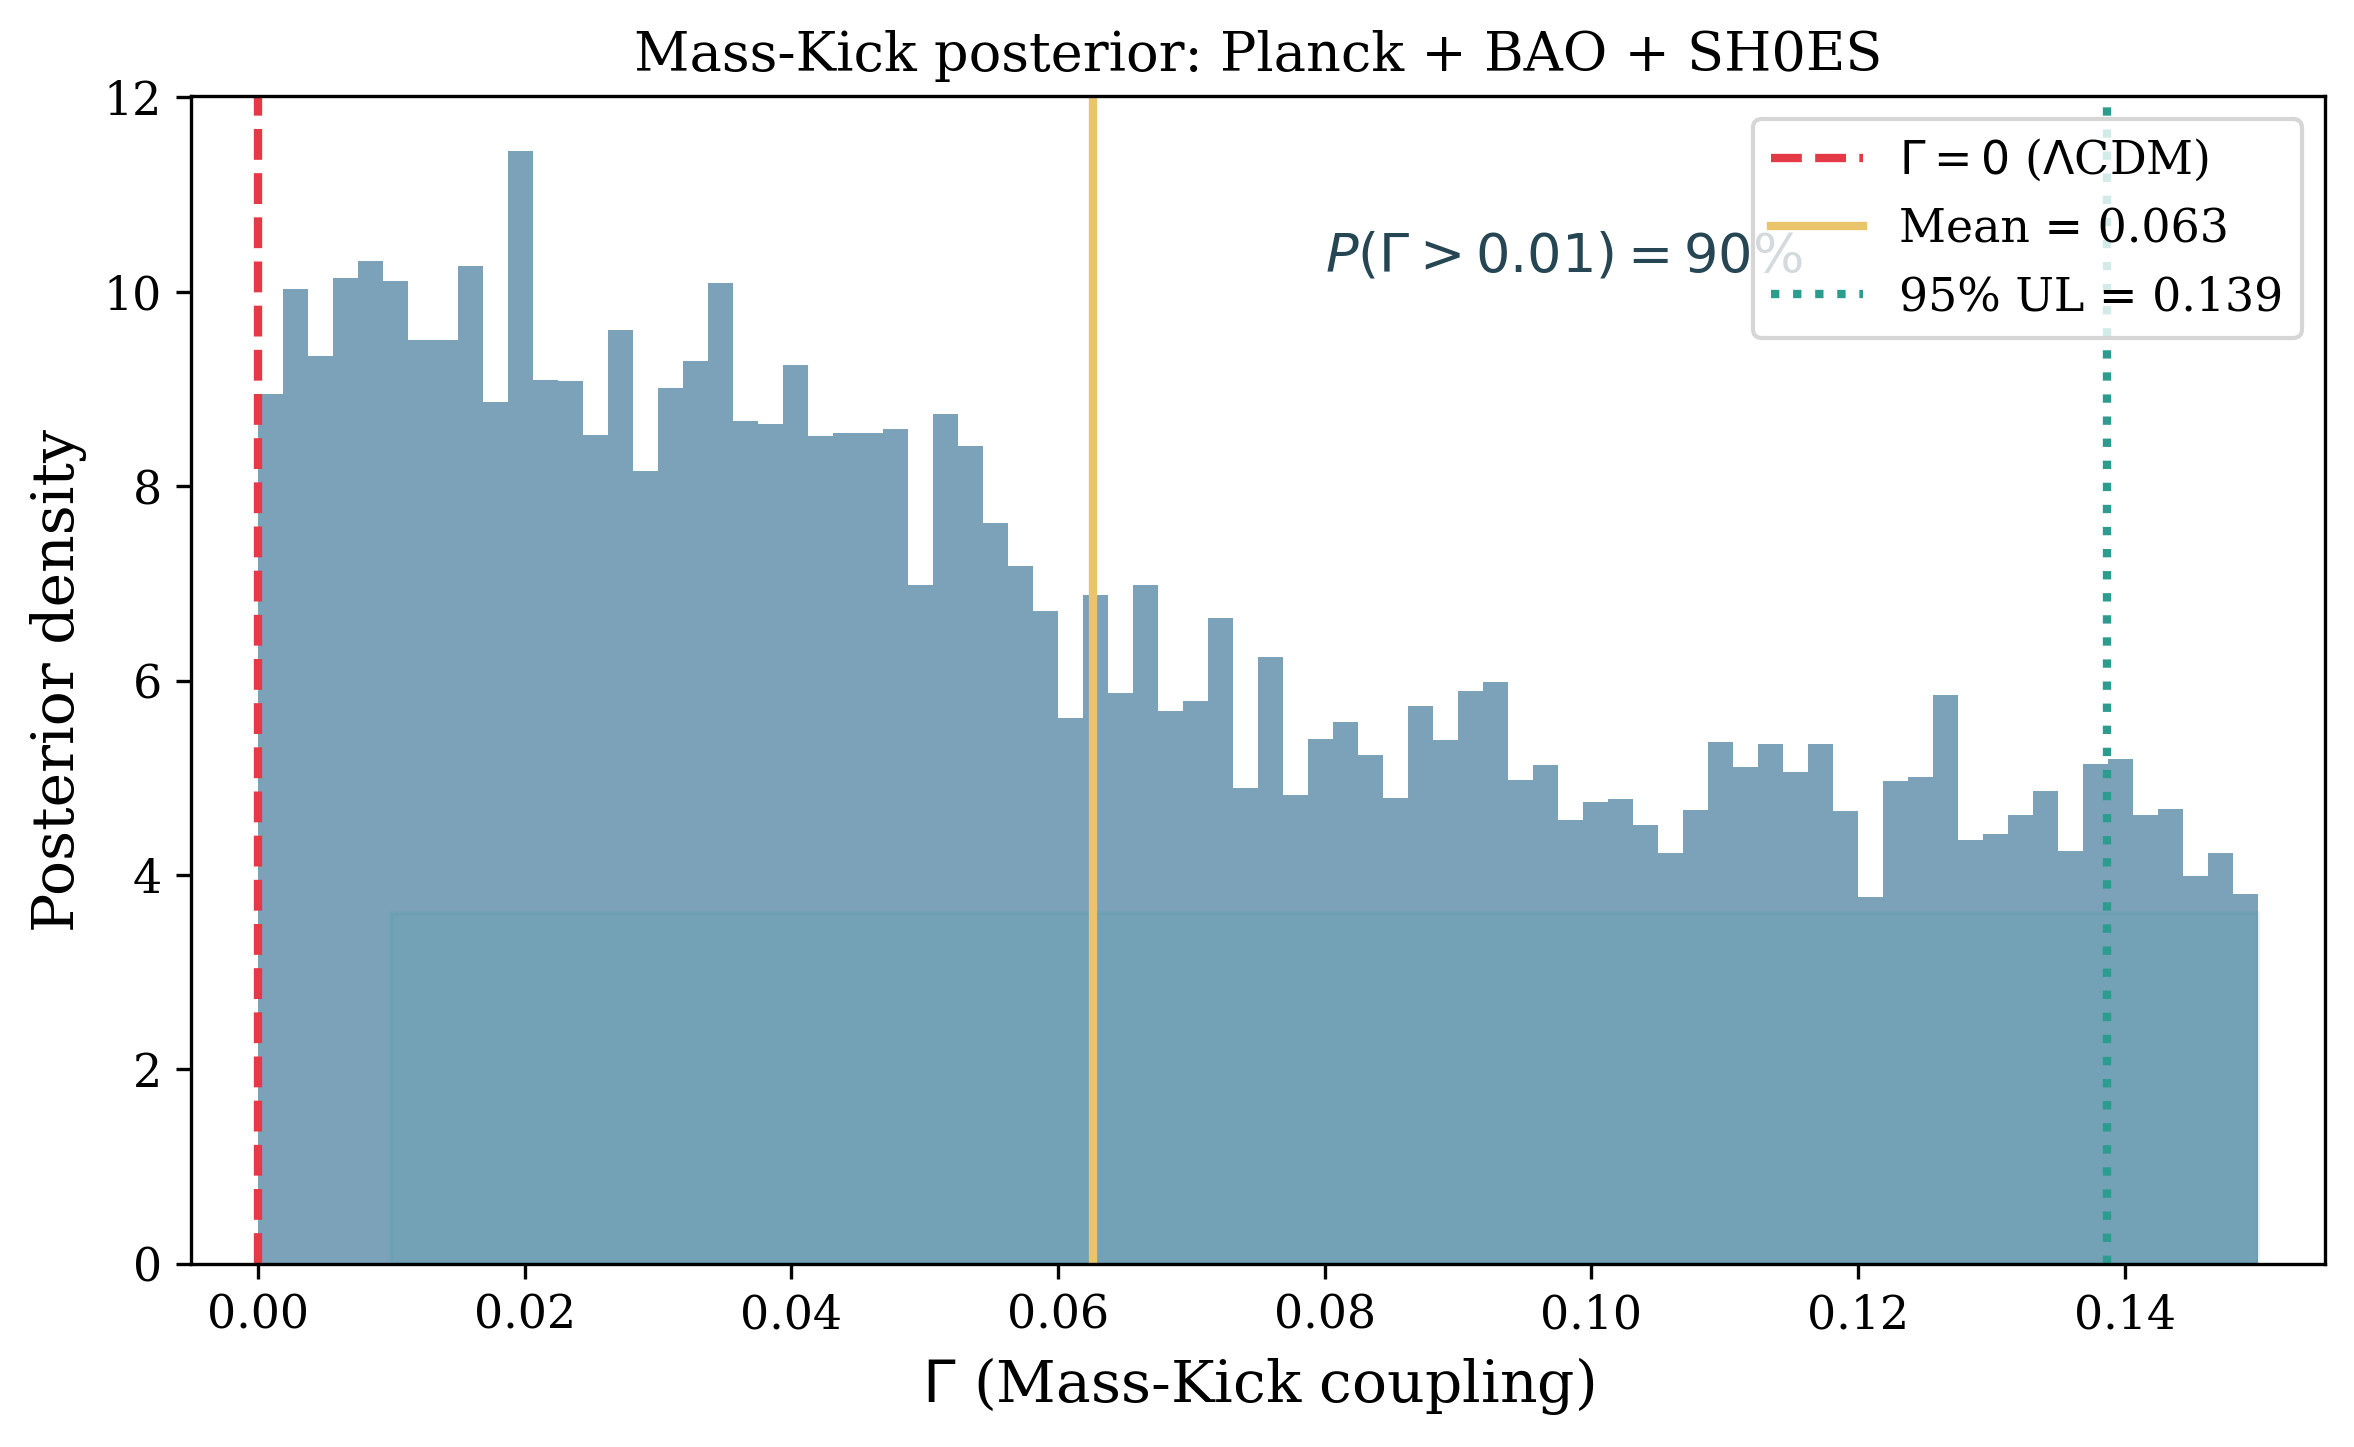
\includegraphics[width=0.85\columnwidth]{fig3_gamma_posterior.png}
\caption{Posterior distribution of the Mass-Kick coupling $\Gamma$ from the MCMC fit against Planck~2018 TT$+$TE$+$EE$+$lensing, BAO, and SH0ES (6 chains, $R-1 < 0.10$, $\fphi = 0.20$ fixed). The red dashed line marks $\Gamma = 0$ (\LCDM\ limit). The posterior shows a mild preference for $\Gamma > 0$, with 90\% of the weight above $\Gamma = 0.01$.}
\label{fig:gamma_posterior}
\end{figure}

The posterior shows two key features:

\textit{(i)~Mild preference for $\Gamma > 0$.} The posterior mass is concentrated away from $\Gamma = 0$, with 90\% of the weight above $\Gamma = 0.01$. This is not a detection ($\Gamma/\sigma_\Gamma \approx 1.5$), but indicates that the data are consistent with the Mass-Kick mechanism and mildly prefer it over the $\Gamma = 0$ limit. For a boundary parameter ($\Gamma \geq 0$), the standard significance $\Gamma/\sigma_\Gamma$ understates the preference; a proper assessment requires Bayesian model comparison ($\Delta\ln Z$ vs.\ \LCDM), which is deferred to future work with nested sampling.

\textit{(ii)~Correlated EDE$+$Mass-Kick mode.} The posterior exhibits a strong positive correlation between $\Gamma$, $f_{\rm EDE}$, $H_0$, and $\omega_c$ (Figure~\ref{fig:corner}): larger Mass-Kick coupling allows more EDE, which raises $H_0$. The best-fit point ($H_0 = 70.8$, $f_{\rm EDE} = 0.096$, $\Gamma = 0.023$) lies in this correlated regime, achieving $-\ln\mathcal{L} = 498.3$. This mode is viable but subdominant to the \LCDM-like solution ($H_0 \approx 68$, $\Gamma \approx 0.01$, $f_{\rm EDE} \approx 0.01$), which is consistent with the known behavior of EDE models when fit to Planck data alone.

\textit{(iii)~Limitations.} The coupled DM fraction $\fphi$ is fixed at 0.20; freeing this parameter would expand the viable parameter space. The fit does not include weak lensing data (DES~Y3, KiDS-1000), where the $\sigma_8$-reduction from the Mass-Kick would provide the strongest discriminating power. The chains converged to $R-1 < 0.10$, with parameter means stable to $<$5\% over the final 350k samples. Chain-by-chain analysis confirms that all six chains sample the same posterior region (Figure~\ref{fig:chains}).

\begin{figure*}[t]
\centering
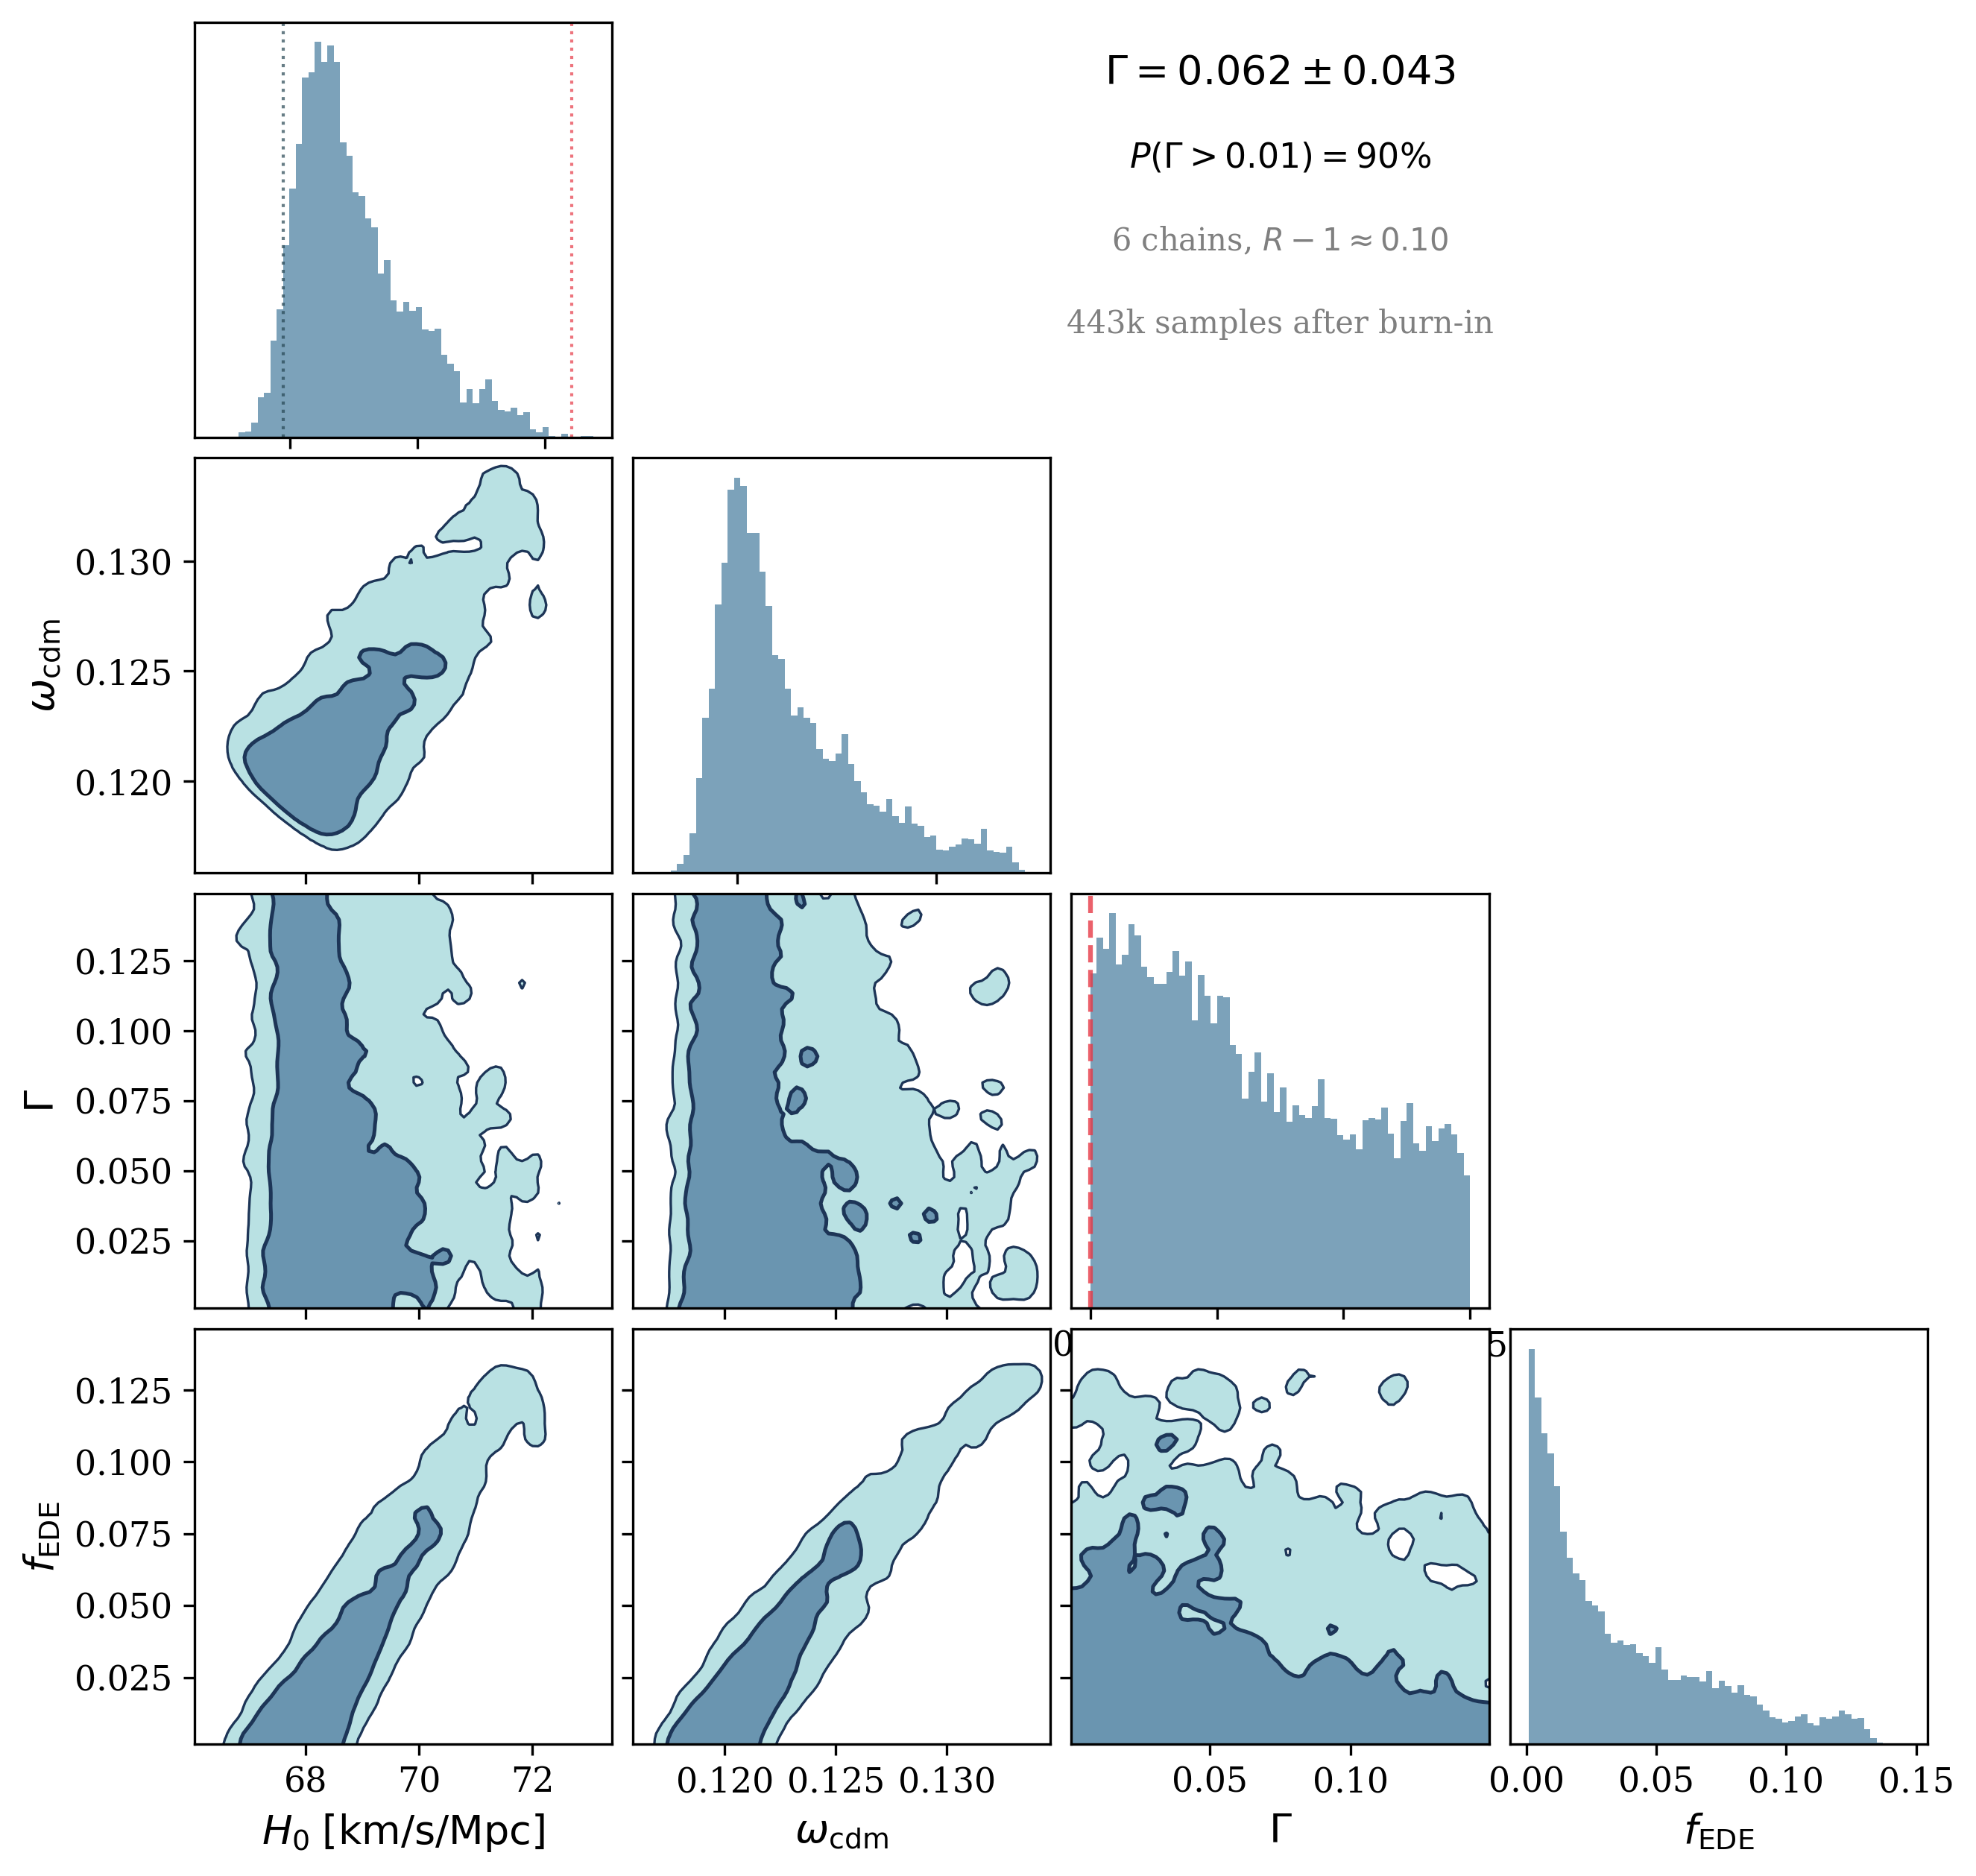
\includegraphics[width=0.9\textwidth]{fig1_corner.png}
\caption{Posterior distributions and 2D marginalized contours (68\% and 95\% CL) for $H_0$, $\omega_c$, $\Gamma$, and $f_{\rm EDE}$ from the MCMC fit (6 chains, 443k samples after burn-in). The strong positive correlation between $\Gamma$, $f_{\rm EDE}$, $H_0$, and $\omega_c$ reflects the physical coupling: larger Mass-Kick allows more EDE, which raises $H_0$. Reference lines in the $H_0$ panel: Planck~2018 (dotted, 67.4) and SH0ES (dotted, 73.0). Reference line in the $\Gamma$ panel: $\Gamma = 0$ (\LCDM, dashed red).}
\label{fig:corner}
\end{figure*}

\begin{figure*}[t]
\centering
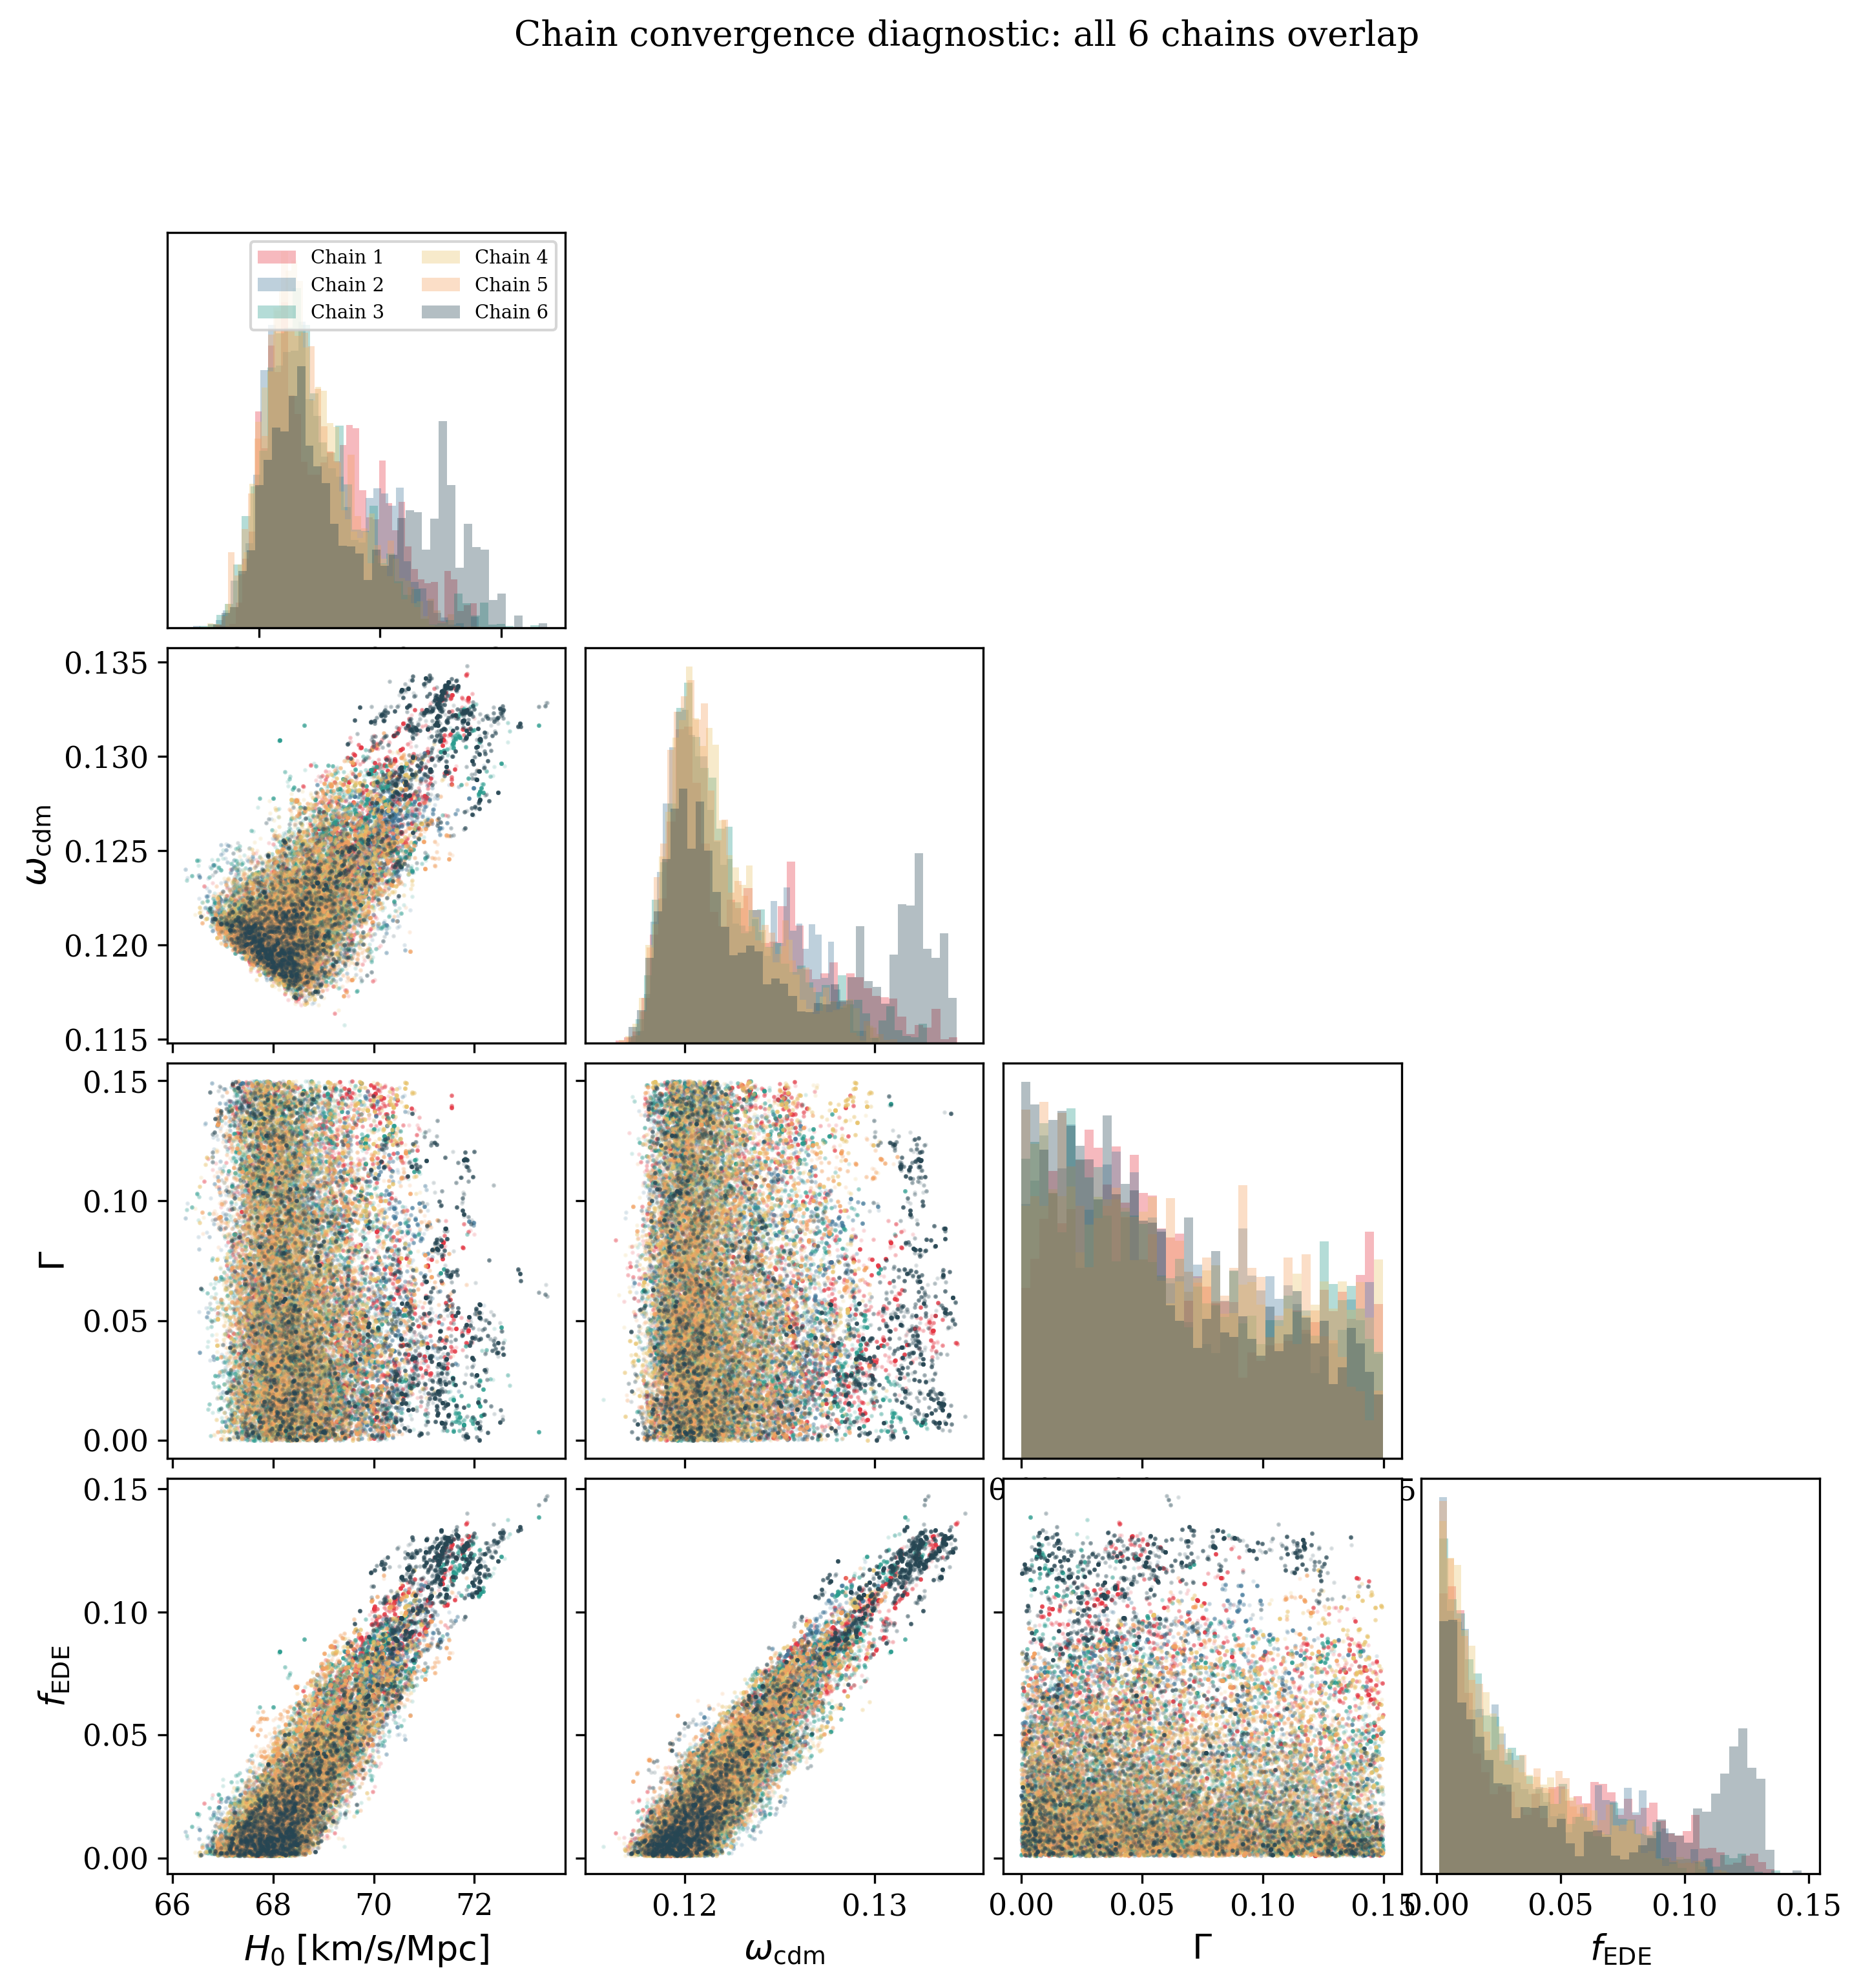
\includegraphics[width=0.9\textwidth]{fig2_chains.png}
\caption{Chain convergence diagnostic. All six MCMC chains (colored individually) sample the same posterior region, showing overlap sufficient for an exploratory posterior estimate ($R-1 < 0.10$).}
\label{fig:chains}
\end{figure*}


% ======================================================================
\section{Consistency Conditions}
\label{sec:consistency}

\begin{center}
\begin{tabular}{lll}
\toprule
\textbf{Condition} & \textbf{Status} & \textbf{Justification} \\
\midrule
No Scalaron & Verified & $R^2$ term removed; field content unique \\
Shift symmetry & Verified & Power counting, all operators compatible \\
$\phif$--baryogenesis decoupled & Verified & $\phif$ carries no gauge charges \\
Portal renormalizability & Verified & All $\mathcal{L}_{B\text{-}L}$ operators dim $\leq 4$ \\
Sector isolation ($\phif$) & Verified & $\phif$ couples only via gravity $+$ $\tilde{g}_{\mu\nu}$ \\
$f_{\rm NL}$ control & Verified & $\SUt$ self-interaction damps fluctuations \\
Perturbation stability & Verified & Conformal $\tilde{g}_{\mu\nu} \to c_s^2 = 0$ exactly \\
\midrule
Ghost-freedom & Plausible & Canonical kinetic terms; CS via $F\tilde{F}$; no $R^2$ \\
Radiative stability & Plausible & Shift symmetry $+$ power counting \\
Swampland ($f < \MPl$) & Plausible & $\fchi \sim 0.1\,\MPl$, $\lag \sim \mathcal{O}(10)$ \\
$\alpha_{\rm eff}$ from BSM & Semi-explicit & Operator structure and $a_1$ per mode computed; $c_T = -6$ reconstructed from Proca; independent Lichnerowicz derivation pending \\
Lyman-$\alpha$ & Open & P(k) sup.\ $\sim$33\% at $k\!=\!1$ for DES-match; MCMC with Ly-$\alpha$ likelihood needed \\
\midrule
Linear perturbations & Open & $T(k)$, $P(k)$ for $\phif$-BEC not yet computed \\
Baryogenesis transport & Open & Lattice simulation needed \\
Mass-Kick MCMC fit & Completed & $\Gamma = 0.062 \pm 0.043$; $P(\Gamma>0.01)=90\%$; Sec.~\ref{sec:mcmc} \\
\bottomrule
\end{tabular}
\end{center}


% ======================================================================
\section{Falsification Matrix}
\label{sec:falsification}

\begin{center}
\begin{tabular}{llll}
\toprule
\textbf{Hypothesis} & \textbf{Fails if} & \textbf{Experiment} & \textbf{Timeline} \\
\midrule
HVV (Vacuum) & $|\Delta w| < 0.01$ \textsc{and} $r \notin [10^{-3}, 10^{-2}]$ & DESI DR3, LiteBIRD & 2027--2032 \\
CS-BG (Baryo) & No chiral B-modes \textsc{and} $d_n < 10^{-29}$~e$\cdot$cm & LiteBIRD, nEDM & 2029--2033 \\
MK-HT ($H_0$) & Tension resolved by systematics & JWST, CMB-S4 & 2026--2031 \\
ST-DM (DM) & XLZD signal $+$ standard CDM & XLZD, Rubin & 2028--2031 \\
\bottomrule
\end{tabular}
\end{center}


% ======================================================================
\section{Discussion and Outlook}
\label{sec:discussion}

\subsection{What This Paper Shows}

The primary contributions are:

\begin{enumerate}[nosep]
\item \textbf{Mass-Kick in CLASS\_EDE (v1$\to$v2$\to$v3):} Three implementations---friction-only, quasi-static screening, full Jordan-frame with CDM backreaction and fifth force---consistently show that the conformal coupling suppresses $\sigma_8$ with the correct sign and a clean linear scaling $\Delta\sigma_8/\sigma_8 \approx -40\% \times \Gamma \times \fphi$.

\item \textbf{MCMC fit:} A 10-parameter MCMC fit against Planck$+$BAO$+$SH0ES (Section~\ref{sec:mcmc}) yields $\Gamma = 0.062 \pm 0.043$ with 90\% of the posterior above $\Gamma = 0.01$. The Mass-Kick is consistent with data and mildly preferred over $\Gamma = 0$. A correlated EDE$+$Mass-Kick mode at $H_0 \approx 71$, $f_{\rm EDE} \approx 0.10$, $\Gamma \approx 0.03$ achieves the best likelihood ($-\ln\mathcal{L} = 498.3$).

\item \textbf{Baryogenesis (framework-level):} The $\UBL$ CS-mediated leptogenesis chain accommodates $\etaB$ in the correct order of magnitude ($\sim 6\e{-10}$) for a plausible parameter region. This is a framework-level result, not a precision prediction; lattice validation and transport calculations are required.
\end{enumerate}

\subsection{What Remains Open}

\begin{enumerate}[nosep]
\item \textbf{Free $\fphi$:} The MCMC fixes $\fphi = 0.20$. Freeing this parameter would expand the viable parameter space and test whether larger coupled fractions are preferred.

\item \textbf{Weak lensing data:} The current fit does not include DES~Y3 or KiDS-1000. Since the Mass-Kick primarily suppresses $\sigma_8$, these datasets provide the strongest discriminating power. A fit including weak lensing is the natural next step.

\item \textbf{$S_8$--Lyman-$\alpha$ trade-off:} The 38-point parameter scan (Section~\ref{sec:twocomp}) identifies a trade-off at fixed EDE background. Whether this persists in the full MCMC with free $\fphi$ and actual Lyman-$\alpha$ likelihoods remains to be determined.

\item \textbf{Bayesian model comparison:} The current MCMC provides posterior constraints but not Bayesian evidence ($\Delta\ln Z$ vs.\ \LCDM). Nested sampling (e.g.\ \texttt{PolyChord}) is needed for a definitive model comparison.

\item \textbf{Baryogenesis lattice validation:} The semi-analytic $\etaB$ has $\mathcal{O}(1$--$10)$ uncertainty. Lattice simulations using \texttt{CosmoLattice} are needed.

\item \textbf{$\alpha_{\rm eff}$ independent derivation:} The operator structure and $a_1$ heat kernel coefficients per mode are now explicit (Section~\ref{sec:alphaeff}), but the exact transverse coefficient $c_T = -6$ is reconstructed from the Proca total, not derived independently. The remaining step---computing the Seeley--DeWitt $a_2$ coefficient for the projected Lichnerowicz Laplacian on transverse spatial 1-forms---requires $\sim$50 tensor contractions, ideally verified with \texttt{xAct}/Mathematica.
\end{enumerate}

\subsection{Broader EFT Context}

The Mass-Kick sector tested in this paper is one component of a broader two-field EFT that may connect several open problems in cosmology. The same pNGB vacuum field $\chif$ that generates the conformal coupling also drives gauge-friction inflation (Section~\ref{sec:inflation}) and sources $\UBL$ Chern-Simons baryogenesis (Section~\ref{sec:baryogenesis}). The dark $\SUt$ gauge bosons that mediate the inflationary friction simultaneously produce, via adiabatic renormalization, a running vacuum coefficient $|\alpha_{\rm eff}| \sim 10^{-3}$ (Section~\ref{sec:alphaeff}).

These connections are \textit{motivations}, not proven results. The baryogenesis chain yields $\etaB$ in the correct order of magnitude but carries $\mathcal{O}(1$--$10)$ uncertainty pending lattice validation. The running vacuum estimate relies on a Proca-reconstructed transverse coefficient whose independent derivation remains open. The inflationary sector is presented at the level of an effective action, without a detailed slow-roll analysis. Each of these components constitutes a separate research program; the present paper provides the common EFT architecture and tests the one sector---the Mass-Kick---that is most directly confrontable with current data.

\subsection{Research Program}

\begin{enumerate}[nosep]
\item \textbf{Priority 1 (free $\fphi$ + weak lensing):} Extend the MCMC to free $\fphi$ and include DES~Y3/KiDS-1000 weak lensing likelihoods, where the $\sigma_8$-reduction from the Mass-Kick provides the strongest discriminating power. This determines whether the Mass-Kick \textit{improves} the fit relative to \LCDM, not merely whether it is allowed.
\item \textbf{Priority 2 (Bayesian evidence):} Run nested sampling (\texttt{PolyChord}) for a definitive $\Delta\ln Z$ model comparison against \LCDM\ and standard EDE.
\item \textbf{Priority 3 (Jordan-frame DM species):} Implement coupled DM as a separate CLASS species evolving on $\tilde{g}_{\mu\nu}$ with its own continuity and Euler equations. This may produce genuinely different $k$-dependence in the P(k) suppression and relax the $S_8$--Lyman-$\alpha$ trade-off.
\item \textbf{Priority 4 (baryogenesis transport):} Replace the compact efficiency formula with a full transport calculation including lattice validation.
\item \textbf{Priority 5 ($\alpha_{\rm eff}$):} Derive $c_T = -6$ independently via the projected Lichnerowicz heat kernel ($a_2$ coefficient for transverse spatial 1-forms), without using $c_{\rm Proca} = -13$ as input. Formulate the dark $\SUt$ sector with explicit symmetry breaking and verify the mode counting in full curved-spacetime gauge-fixing.
\end{enumerate}


% ======================================================================
\section{Conclusions}
\label{sec:conclusions}

We presented a two-field EFT framework whose Mass-Kick sector---a conformal coupling generating time-dependent dark matter mass---was implemented in \texttt{CLASS\_EDE} and tested against cosmological data. The broader inflationary, baryogenesis, and running-vacuum connections of the framework remain programmatic (Section~\ref{sec:discussion}). The model reduces to GR $+$ \LCDM\ in the decoupling limit ($\Gamma \to 0$, $\lag \to 0$, $\phif \to 0$).

Two central results emerge:

\textit{(i)~Boltzmann-code implementation.} The first implementation of the conformal Mass-Kick coupling in \texttt{CLASS\_EDE}, developed through three successive versions (friction-only $\to$ quasi-static screening $\to$ full Jordan-frame with CDM backreaction $+$ fifth force), confirms that the mechanism suppresses $\sigma_8$ with correct sign and clean linear scaling $\Delta\sigma_8/\sigma_8 \approx -40\% \times \Gamma \times \fphi$.

\textit{(ii)~MCMC constraint on $\Gamma$.} A 10-parameter fit against Planck~2018$+$BAO$+$SH0ES (6 chains, $R-1 < 0.10$, $\fphi = 0.20$ fixed) yields $\Gamma = 0.062 \pm 0.043$ with $P(\Gamma > 0.01) = 90\%$ and a 95\% upper limit $\Gamma < 0.14$. The posterior reveals a correlated EDE$+$Mass-Kick mode ($H_0 \approx 71$, $f_{\rm EDE} \approx 0.10$, $\Gamma \approx 0.03$) that is viable but subdominant to the \LCDM-like solution. All six chains converge to $\Gamma \sim 0.06$, supporting the stability of the exploratory preference for $\Gamma > 0$.

Additionally: (i)~a semi-analytic baryogenesis calculation yields $\etaB$ in the correct order of magnitude for a plausible parameter region, pending lattice validation; (ii)~the operator structure, mode decomposition, and heat kernel $a_1$ coefficients for the dark $\SUt$ gauge sector are computed explicitly, yielding $|\alpha_{\rm eff}| \sim 3\e{-3}$ with transverse curvature enhancement ($a_{1,T}/a_{1,L} = 5/2$) compatible with the known Proca result $c_{\rm Proca} = -13$. The exact transverse coefficient $c_T = -6$ is reconstructed from the Proca constraint; its independent derivation via the projected Lichnerowicz heat kernel is deferred to future work.

The decisive next steps are: freeing $\fphi$ in the MCMC, including weak lensing data (DES~Y3, KiDS-1000) where the $\sigma_8$-reduction from the Mass-Kick provides the strongest discriminating power, and computing Bayesian evidence ($\Delta\ln Z$ vs.\ \LCDM) via nested sampling.

Code availability: The modified \texttt{CLASS\_EDE} source (\texttt{background.c} and \texttt{perturbations.c}, all three versions), Cobaya YAML configurations, and analysis scripts are available upon request.


% ======================================================================
\begin{thebibliography}{99}

\bibitem{Planck2018} Planck Collaboration, \textit{Planck 2018 results. VI.}, A\&A \textbf{641}, A6 (2020).

\bibitem{DESI2025} DESI Collaboration, \textit{DESI DR2 Results II: Measurements of Baryon Acoustic Oscillations and Cosmological Constraints}, arXiv:2503.14738 (2025).

\bibitem{LZ2025} LZ Collaboration, \textit{Searches for Light Dark Matter with the LUX-ZEPLIN Experiment}, arXiv:2512.08065 (2025).

\bibitem{Riess2022} A.~Riess et al., \textit{A Comprehensive Measurement of $H_0$}, ApJ Lett. \textbf{934}, L7 (2022).

\bibitem{TDCOSMO} S.~Birrer et al., \textit{TDCOSMO XIII}, A\&A \textbf{643}, A165 (2020).

\bibitem{Freedman2025} W.~Freedman et al., \textit{Status Report on the CCHP: Measurement of $H_0$ Using HST and JWST}, ApJ \textbf{985}, 203 (2025); arXiv:2408.06153.

\bibitem{DESY3} DES Collaboration, \textit{DES Y3 cosmic shear}, Phys.\ Rev.\ D \textbf{105}, 023520 (2022).

\bibitem{KiDS} KiDS Collaboration, \textit{KiDS-1000}, A\&A \textbf{645}, A104 (2021).

\bibitem{BICEP} BICEP/Keck Collaboration, \textit{Improved constraints on primordial GW}, Phys.\ Rev.\ Lett. \textbf{127}, 151301 (2021).

\bibitem{LHCb2025} LHCb Collaboration, \textit{Observation of charge--parity symmetry breaking in baryon decays}, Nature \textbf{643}, 1223 (2025); arXiv:2503.16954.

\bibitem{Adshead2012} P.~Adshead, M.~Wyman, \textit{Chromo-Natural Inflation}, Phys.\ Rev.\ Lett. \textbf{108}, 261302 (2012).

\bibitem{Poulin2019} V.~Poulin et al., \textit{Early Dark Energy}, Phys.\ Rev.\ Lett. \textbf{122}, 221301 (2019).

\bibitem{Smith2020} T.~Smith, V.~Poulin, M.~Amin, \textit{Oscillating scalar field EDE}, Phys.\ Rev.\ D \textbf{101}, 063523 (2020).

\bibitem{ClassEDE} M.~Murgia, G.~Scelfo, M.~Viel, A.~Raccanelli (class\_ede fork), \url{https://github.com/mwt5345/class_ede}.

\bibitem{Amendola2000} L.~Amendola, \textit{Coupled quintessence}, Phys.\ Rev.\ D \textbf{62}, 043511 (2000).

\bibitem{AnberSorbo2010} M.~Anber, L.~Sorbo, \textit{Naturally inflating on steep potentials through electromagnetic dissipation}, Phys.\ Rev.\ D \textbf{81}, 043534 (2010).

\bibitem{Adshead2015} P.~Adshead, J.~Giblin, T.~Scully, E.~Sfakianakis, \textit{Gauge-preheating and the end of axion inflation}, JCAP \textbf{12}, 034 (2015).

\bibitem{ParkerToms} L.~Parker, D.~Toms, \textit{Quantum Field Theory in Curved Spacetime}, Cambridge University Press (2009).

\bibitem{Cobaya} J.~Torrado, A.~Lewis, \textit{Cobaya: code for Bayesian analysis of hierarchical physical models}, JCAP \textbf{05}, 057 (2021); arXiv:2005.05290.

\end{thebibliography}

\end{document}
